\documentclass[11pt]{article}
\usepackage[margin=0.8in]{geometry}
\usepackage{lmodern,microtype,booktabs,graphicx,amsmath,xcolor,hyperref,xurl}
\hypersetup{colorlinks=true,urlcolor=blue,linkcolor=blue,pdftitle={Check the simple baseline before refitting a cache forecast},pdfauthor={James N. Jean IV}}
\setlength{\parindent}{0pt}\setlength{\parskip}{6pt}
\setlength{\tabcolsep}{5pt}
\newcommand{\MSourceObjects}{6}
\newcommand{\MSourceBytes}{126,293,595}
\newcommand{\MSourceConditions}{1,200,060}
\newcommand{\MRequests}{1,200,000}
\newcommand{\MDevConditions}{603,643}
\newcommand{\MFinalConditions}{1,806,171}
\newcommand{\MDevPredictions}{480}
\newcommand{\MFinalPredictions}{720}
\newcommand{\MTrain}{351}
\newcommand{\MValidation}{120}
\newcommand{\MFinalOrigins}{360}
\newcommand{\MChangedOrigins}{240}
\newcommand{\MTransientOrigins}{30}
\newcommand{\MDeps}{47}
\newcommand{\MLambda}{0.01}
\newcommand{\MDevBase}{0.073100}
\newcommand{\MDevLinear}{0.081148}
\newcommand{\MControlBase}{0.047275}
\newcommand{\MControlLinear}{0.064059}
\newcommand{\MShrinkBase}{0.048117}
\newcommand{\MShrinkLinear}{0.066809}
\newcommand{\MExpandBase}{0.061842}
\newcommand{\MExpandLinear}{0.074959}
\newcommand{\MChangedPrimaryBase}{0.054979}
\newcommand{\MChangedPrimaryLinear}{0.070884}
\newcommand{\MChangedFirstFiveBase}{0.072467}
\newcommand{\MChangedFirstFiveLinear}{0.076499}
\newcommand{\MChangedBaseMSE}{0.012023}
\newcommand{\MChangedBaseBias}{-0.004112}
\newcommand{\MChangedBaseClipped}{0}
\newcommand{\MChangedLinearMSE}{0.011782}
\newcommand{\MChangedLinearBias}{-0.014050}
\newcommand{\MChangedLinearClipped}{0}
\newcommand{\MDelta}{0.015905}
\newcommand{\MTraceABytes}{18,681,259}
\newcommand{\MTraceADistinct}{58,916}
\newcommand{\MTraceARecords}{200,000}
\newcommand{\MTraceBBytes}{31,418,669}
\newcommand{\MTraceBDistinct}{169,486}
\newcommand{\MTraceBRecords}{200,000}
\newcommand{\MTraceCBytes}{23,351,435}
\newcommand{\MTraceCDistinct}{79,090}
\newcommand{\MTraceCRecords}{200,000}
\newcommand{\MTraceDBytes}{20,130,322}
\newcommand{\MTraceDDistinct}{46,523}
\newcommand{\MTraceDRecords}{200,000}
\newcommand{\MTraceEBytes}{14,222,241}
\newcommand{\MTraceEDistinct}{199,776}
\newcommand{\MTraceERecords}{200,000}
\newcommand{\MTraceFBytes}{18,489,669}
\newcommand{\MTraceFDistinct}{53,643}
\newcommand{\MTraceFRecords}{200,000}
\newcommand{\MGroupABase}{0.116725}
\newcommand{\MGroupALinear}{0.124960}
\newcommand{\MGroupBBase}{0.023950}
\newcommand{\MGroupBLinear}{0.038586}
\newcommand{\MGroupCBase}{0.001150}
\newcommand{\MGroupCLinear}{0.028630}
\newcommand{\MGroupDBase}{0.132675}
\newcommand{\MGroupDLinear}{0.139946}
\newcommand{\MGroupEBase}{0.011425}
\newcommand{\MGroupELinear}{0.031799}
\newcommand{\MGroupFBase}{0.000250}
\newcommand{\MGroupFLinear}{0.028683}
\newcommand{\MGroupGBase}{0.097075}
\newcommand{\MGroupGLinear}{0.107512}
\newcommand{\MGroupHBase}{0.083950}
\newcommand{\MGroupHLinear}{0.088386}
\newcommand{\MGroupIBase}{0.004500}
\newcommand{\MGroupILinear}{0.028979}
\begin{document}
\begin{center}
{\LARGE\bfseries Check the simple baseline\\before refitting a cache forecast}\par
\vspace{8pt}James N. Jean IV\\
Independent research and implementation study\quad 30 October 2026\\
{\small Reproducible trace exercise, not peer reviewed}
\end{center}
\section*{Decision brief}
Changing a cache configuration can change the miss fraction that a planner is trying to forecast. This study compares a selected linear forecast with a previous-block baseline after authored capacity changes on recorded request prefixes.

The previous-block baseline has lower mean absolute error (MAE) in all nine final volume/scenario groups, including unchanged controls. Across the six changed groups, MAE is \MChangedPrimaryBase{} versus \MChangedPrimaryLinear{} for the frozen linear model, a gap of \MDelta{} miss-fraction units. Development already favored the baseline. Cache changes alone therefore do not explain the linear model's weakness.

The loss metric matters: combined changed-group mean squared error (MSE) favors the linear model, \MChangedLinearMSE{} versus \MChangedBaseMSE{}. The recommendation below concerns the predeclared MAE objective, not an overall win on every measure.

\begin{center}\begin{tabular}{lrr}\toprule
Final macro MAE, lower is better & Previous block & Frozen linear\\\midrule
512 unchanged & \MControlBase & \MControlLinear \\
512 to 128 & \MShrinkBase & \MShrinkLinear \\
512 to 2,048 & \MExpandBase & \MExpandLinear \\
Changed combined & \MChangedPrimaryBase & \MChangedPrimaryLinear \\
First five, changed & \MChangedFirstFiveBase & \MChangedFirstFiveLinear \\
\bottomrule\end{tabular}\end{center}

\textbf{Practical recommendation.} Keep a simple baseline and configuration boundaries in the evaluation before investing in a more complex forecast. Under the predeclared MAE objective, this benchmark does not justify replacing the previous-block baseline with the tested linear model. A real deployment needs prospective, byte-aware measurement and operating costs.

\textbf{What the numbers mean.} A target is the simulated miss fraction in the next 1,000 recorded requests under equal-object LRU. A slot is an abstract object position, not RAM bytes. These are neither production miss measurements nor clock-time IOPS, latency, throughput, energy or savings.

\textbf{Scope.} Six converted 2007 storage traces are selected by file-size metadata before values; fixed prefixes supply three development and three final volumes. The final set includes two volumes with the same server label. Prefixes and scenarios are dependent convenience samples. No novelty, adoption, deployment benefit or causal generalization to production is established.
\newpage
\section*{1. Recorded data, transformed without future access}
The open-source cache collection explicitly identifies CC BY 4.0 and credits Juncheng Yang for curation/conversion. The original Microsoft Cambridge study is Narayanan, Donnelly and Rowstron's FAST 2008 paper on write off-loading. Its power-management findings are not findings of this exercise.

Before acquisition, the observed converted OracleGeneral folder's fourteen objects were sorted by displayed MB size, ties by filename; the smallest six were fixed. The collection README's thirteen-trace summary is not reconciled with the observed fourteen-object folder. Six metadata HEAD reads establish exact lengths and ETags. \MSourceObjects{} subsequent GETs capture \MSourceBytes{} compressed bytes without redirects, retries or denied responses.

\begin{center}\small\begin{tabular}{llrrr}\toprule
Trace & Group & Compressed bytes & Prefix identities & Requests\\\midrule
msr\_hm\_0 & development & \MTraceABytes & \MTraceADistinct & \MTraceARecords \\
msr\_usr\_2 & final & \MTraceBBytes & \MTraceBDistinct & \MTraceBRecords \\
msr\_prn\_0 & development & \MTraceCBytes & \MTraceCDistinct & \MTraceCRecords \\
msr\_proj\_4 & final & \MTraceDBytes & \MTraceDDistinct & \MTraceDRecords \\
msr\_web\_2 & development & \MTraceEBytes & \MTraceEDistinct & \MTraceERecords \\
msr\_proj\_0 & final & \MTraceFBytes & \MTraceFDistinct & \MTraceFRecords \\
\bottomrule\end{tabular}\end{center}

Each file contributes its first 200,000 complete 24-byte records, giving \MRequests{} transformed requests. The official reader establishes object bytes 4:12 and future-access bytes 16:24. The projection treats object tokens as opaque bytes and assigns an ordinal at first appearance. It never decodes future access. Public sequences exclude per-request raw addresses, clocks, sizes and future values.

Clock/size quality fields use a recorded little-endian working interpretation, without an asserted calendar-time unit. All prefixes have nondecreasing raw clocks; ties and all requests remain. Fixed request counts cover differing source spans and cannot be treated as equal elapsed time. No request thinning, interpolation, outcome-selected prefix or volume dropping occurs.

Exact complete compressed objects remain private, with local SHA256 identities and safe headers; multipart S3 ETags are not SHA256 checksums. Only fixed prefixes are semantically inspected. An independent byte parser reconciles every ordinal and quality field in \MSourceConditions{} conditions. CC BY 4.0 attribution and the prefix/remapping/simulation modifications are explicit.
\newpage
\section*{2. Fixed models and configuration separation}
Each prefix has 200 blocks of 1,000 requests. Simulations begin cold with 512 equal-object LRU slots. Development fits on blocks 3--119 of three volumes (\MTrain{} origins) and validates on blocks 120--159 (\MValidation{} origins). Inputs are only the three prior completed miss fractions; the target block, capacity indicator, future-access field, source sizes and full-trace summaries are excluded.

With an intercept and three lag features, the exact rational fit solves
\[
 \bigl(X^\top X+\lambda\,\mathrm{diag}(0,1,1,1)\bigr)\beta=X^\top y.
\]
There is no scaling or hidden optimizer. The intercept is unpenalized. The normal-equation penalty is $\lambda$, not $\lambda n$. All three authored values $0.01,1,100$ and predictions are retained; forecasts are clipped to $[0,1]$ with raw values preserved.

\begin{center}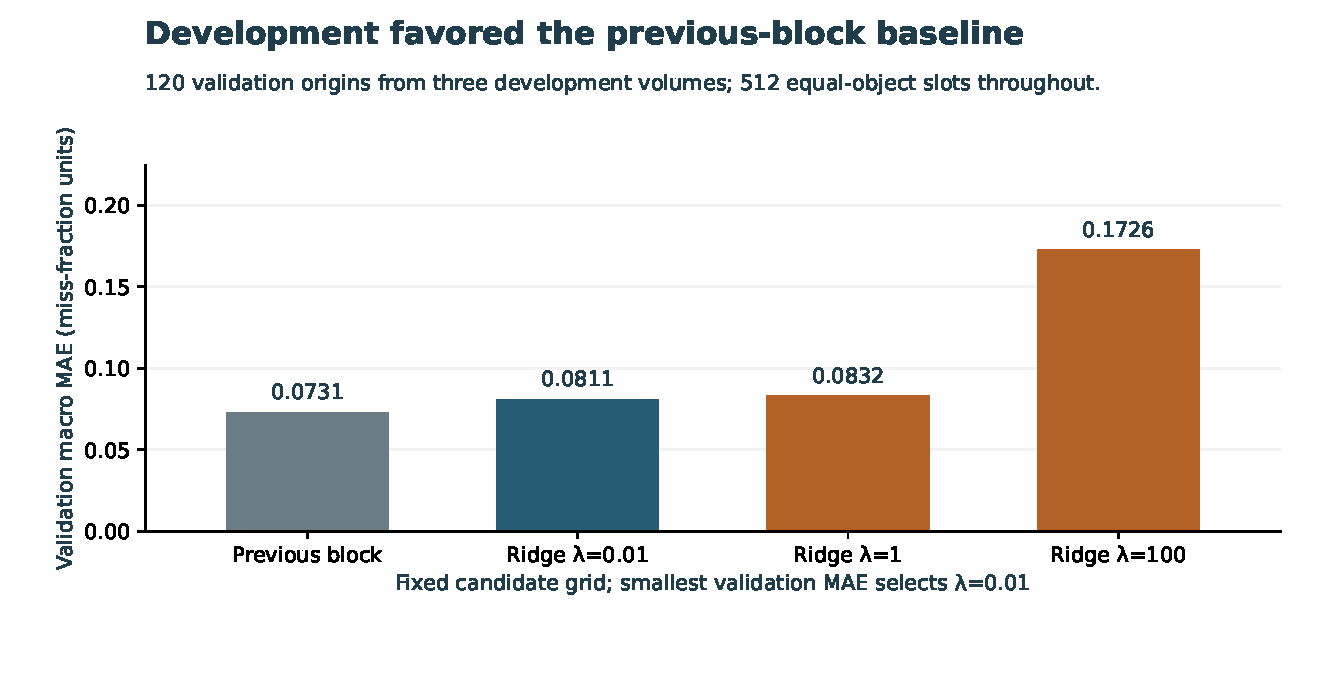
\includegraphics[width=\linewidth]{images/validation_search.pdf}\end{center}

Selection minimizes exact validation MAE averaged equally across development volumes; exact ties prefer larger penalty. The selected $\lambda=\MLambda$ is the lower grid boundary. Its validation MAE \MDevLinear{} is worse than the baseline's \MDevBase{}. The grid is not expanded and there is no validation refit.

A committed manifest of \MDeps{} dependencies precedes all final-volume simulation, features and scores. Source request IDs are already present, so collection is not blinded. This is a protected analytical evaluation, not an original-vintage production forecast.
\newpage
\section*{3. Final volumes and later request blocks}
Other volumes use blocks 160--199, with \MFinalOrigins{} origins per model across three scenarios. Through block 159 all scenarios share capacity 512 and resident state. Before block 160, control stays 512, shrink moves to 128 and expansion to 2,048. Shrinking evicts oldest entries immediately; expansion does not resurrect prior evictions. No cold restart occurs at the change.

\begin{center}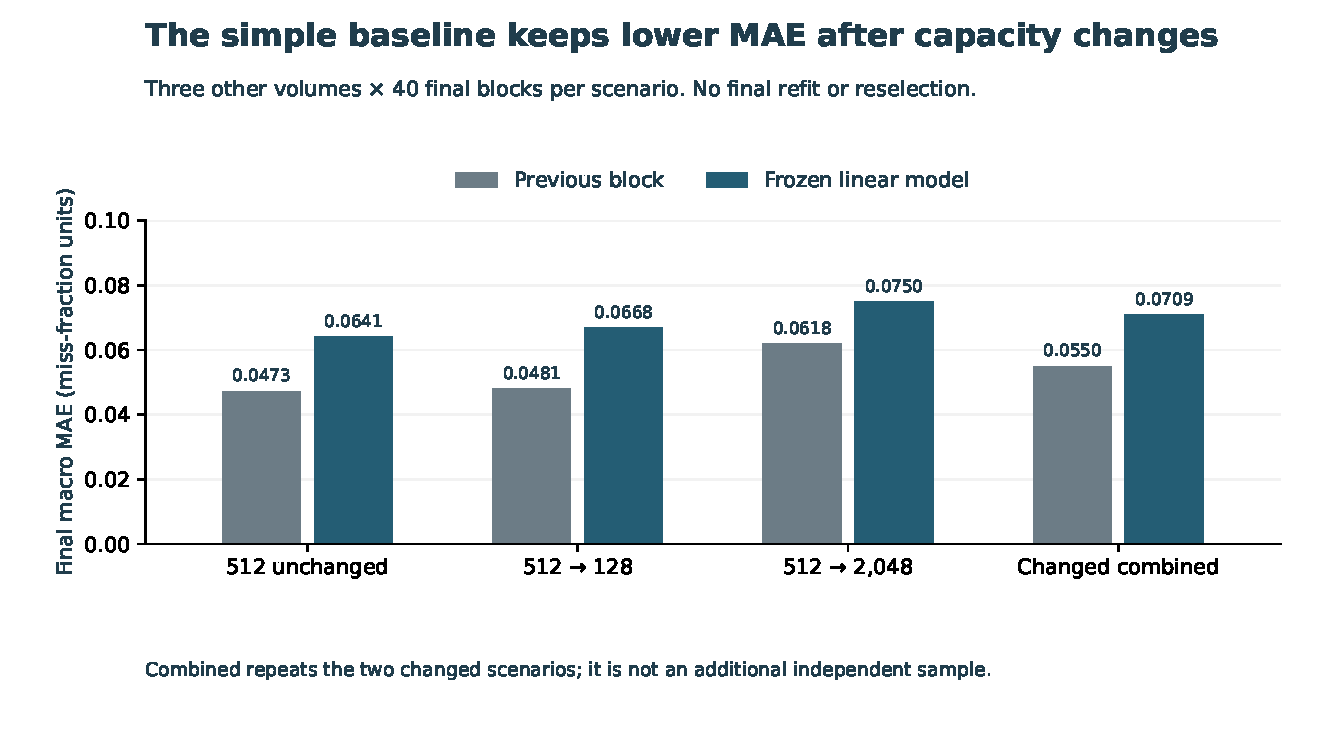
\includegraphics[width=\linewidth]{images/final_scenarios.pdf}\end{center}

\begin{center}\small\begin{tabular}{llrr}\toprule
Volume & Scenario & Previous-block MAE & Linear MAE\\\midrule
msr\_proj\_0 & control & \MGroupABase & \MGroupALinear \\
msr\_proj\_4 & control & \MGroupBBase & \MGroupBLinear \\
msr\_usr\_2 & control & \MGroupCBase & \MGroupCLinear \\
msr\_proj\_0 & shrink & \MGroupDBase & \MGroupDLinear \\
msr\_proj\_4 & shrink & \MGroupEBase & \MGroupELinear \\
msr\_usr\_2 & shrink & \MGroupFBase & \MGroupFLinear \\
msr\_proj\_0 & expand & \MGroupGBase & \MGroupGLinear \\
msr\_proj\_4 & expand & \MGroupHBase & \MGroupHLinear \\
msr\_usr\_2 & expand & \MGroupIBase & \MGroupILinear \\
\bottomrule\end{tabular}\end{center}

The baseline has lower MAE in each displayed group, including controls. The combined changed comparison has \MChangedOrigins{} origins in six dependent groups; its first-five-block view has \MTransientOrigins{}. Combined rows repeat component observations rather than add an independent sample. No final outcome chooses a new penalty, feature, boundary or configuration.

Changed-group macro MSE is \MChangedBaseMSE{} for the baseline and \MChangedLinearMSE{} for the linear model. Mean signed error (prediction minus target) is \MChangedBaseBias{} versus \MChangedLinearBias{}. Clipped final changed predictions number \MChangedBaseClipped{} and \MChangedLinearClipped{}, respectively.
\newpage
\section*{4. Keep the known change visible}
\begin{center}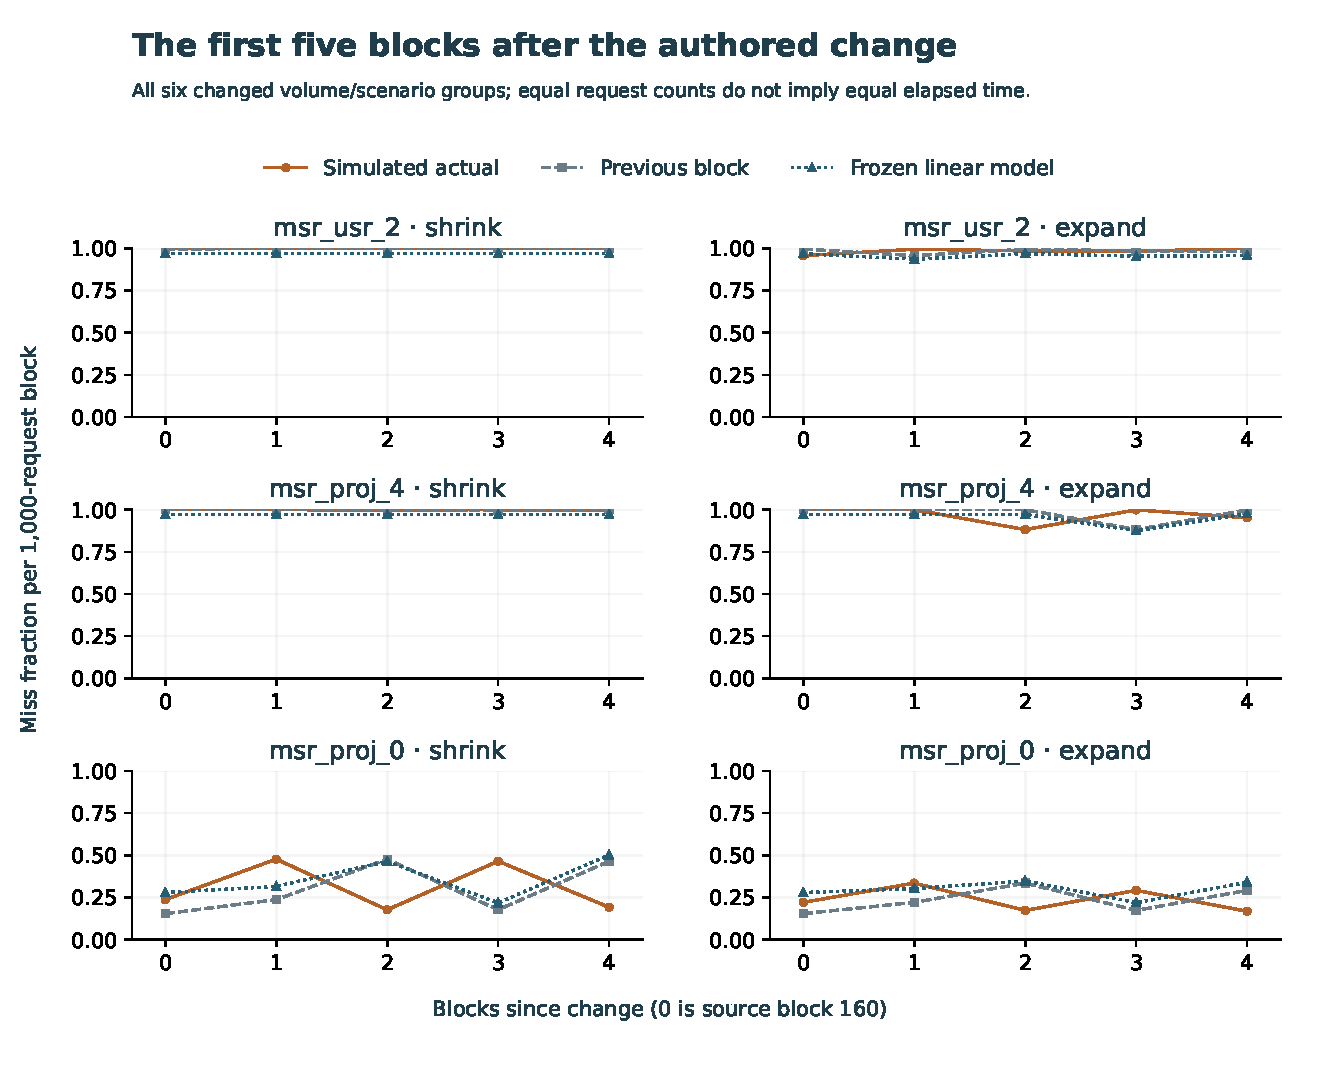
\includegraphics[width=\linewidth]{images/change_transients.pdf}\end{center}

The first post-change forecast receives identical past features across each volume's three scenarios; the model does not receive a capacity indicator. Later forecasts can adapt through newly observed miss fractions. This deliberately configuration-blind setup tests transfer; it does not recommend hiding a known operational change.

The offline exercise accepts three authored completed miss counts, newest first, plus declared change context. It returns baseline and frozen-model estimates with a reminder to collect post-change history. Missing history remains UNKNOWN.
\begin{verbatim}
python src/review_cli.py examples/authored-changed-context.json
python src/review_cli.py examples/unknown-history.json
\end{verbatim}
The exercise changes no cache, sends no alert and makes no source request. Its estimates are teaching outputs. A deployment study should include byte occupancy, I/O operations, timing, concurrency, actual cache policy and measured costs before selecting capacity or claiming operational improvement.
\newpage
\section*{5. Independent checks and reproducibility}
The main simulator uses OrderedDict. A separate resident dictionary and min-heap implementation checks all request misses and block counts, including preserved resize state. SQLite lag windows independently reconstruct feature boundaries. Exact Fraction fitting and metrics are checked against a separate NumPy 2.2.5 normal-equation solve; coefficient, prediction and metric absolute tolerances are $10^{-8}$, $10^{-9}$ and $10^{-10}$. Saved rational metrics and selection also match exactly.

Development retains \MDevPredictions{} predictions and passes \MDevConditions{} conditions, including 600,000 request misses. Final retains \MFinalPredictions{} predictions and passes \MFinalConditions{} conditions, including 1,800,000 request misses across nine simulations. Twenty-seven fixture methods cover cold starts, recency, shrink, expansion without resurrection, request-block boundaries, source truncation, future-byte mutation invariance, no-future features, constant fits, exact ties, clipping and exercise input.

\begin{verbatim}
python -m unittest discover -s tests -v
python src/freeze_proof.py
python src/replay.py --output ../fresh-replay
python src/verify_figures.py
\end{verbatim}
Use a full-history clone and fresh external output. Replay recomputes simulations and forecasts from saved ordinal prefixes, checks source/frozen bytes and writes new runtime receipts separately. It makes no source request. Gzip outputs compare as logical JSON, avoiding irrelevant cross-runtime header differences. Release requires two-runtime isolated replay, actual SVG coordinates/hashes, all rendered paper pages, a scoped publication audit, exact candidate/main Linux CI, matching tree and a remote annotated tag.

\section*{Primary references and provenance}
\small
Juncheng Yang. \emph{Open-source Cache Dataset}. \url{https://github.com/cacheMon/cache_dataset}. Collection and converted trace license: CC BY 4.0, \url{https://creativecommons.org/licenses/by/4.0/}. Prefix selection and key remapping are modifications; no endorsement is implied.

Dushyanth Narayanan, Austin Donnelly and Antony Rowstron. \emph{Write Off-Loading: Practical Power Management for Enterprise Storage}. FAST 2008. \url{https://www.usenix.org/legacy/event/fast08/tech/full_papers/narayanan/narayanan.pdf}.

libCacheSim. \emph{OracleGeneral binary reader}. \url{https://github.com/1a1a11a/libCacheSim}. Inspected field-layout blob \nolinkurl{6cfaf0b87c7a17b1458428a57d85b3e3002fe2f9}. Only format facts are used; external code is not executed.

James N. Jean IV. \emph{Cache-change forecast audit}. \url{https://github.com/S3R3Bii/cache-change-forecast-audit}. Independent trace benchmark and offline exercise, not peer reviewed. Formal-publication projects, including Azure optimization, remain private.
\end{document}
